\chapter{Diseño e Implementación} % Main chapter title

\label{Chapter3} % Change X to a consecutive number; for referencing this chapter elsewhere, use \ref{ChapterX}
\definecolor{mygreen}{rgb}{0,0.6,0}
\definecolor{mygray}{rgb}{0.5,0.5,0.5}
\definecolor{mymauve}{rgb}{0.58,0,0.82}

\lstset{ %
  backgroundcolor=\color{white},   % choose the background color; you must add \usepackage{color} or \usepackage{xcolor}
  basicstyle=\footnotesize,        % the size of the fonts that are used for the code
  breakatwhitespace=false,         % sets if automatic breaks should only happen at whitespace
  breaklines=true,                 % sets automatic line breaking
  captionpos=b,                    % sets the caption-position to bottom
  commentstyle=\color{mygreen},    % comment style
  deletekeywords={...},            % if you want to delete keywords from the given language
  %escapeinside={\%*}{*)},          % if you want to add LaTeX within your code
  %extendedchars=true,              % lets you use non-ASCII characters; for 8-bits encodings only, does not work with UTF-8
  %frame=single,	                   % adds a frame around the code
  keepspaces=true,                 % keeps spaces in text, useful for keeping indentation of code (possibly needs columns=flexible)
  keywordstyle=\color{blue},       % keyword style
  language=[ANSI]C,					% the language of the code
  %otherkeywords={*,...},           % if you want to add more keywords to the set
  numbers=left,                    % where to put the line-numbers; possible values are (none, left, right)
  numbersep=5pt,                   % how far the line-numbers are from the code
  numberstyle=\tiny\color{mygray}, % the style that is used for the line-numbers
  rulecolor=\color{black},         % if not set, the frame-color may be changed on line-breaks within not-black text (e.g. comments (green here))
  showspaces=false,                % show spaces everywhere adding particular underscores; it overrides 'showstringspaces'
  showstringspaces=false,          % underline spaces within strings only
  showtabs=false,                  % show tabs within strings adding particular underscores
  stepnumber=1,                    % the step between two line-numbers. If it's 1, each line will be numbered
  stringstyle=\color{mymauve},     % string literal style
  tabsize=2,	                   % sets default tabsize to 2 spaces
  title=\lstname,                   % show the filename of files included with \lstinputlisting; also try caption instead of title
  morecomment=[s]{/*}{*/}%
}


%----------------------------------------------------------------------------------------
%	SECTION 1
%----------------------------------------------------------------------------------------
\section{Diseño e Implementación}
En este capítulo se mostrará cómo se desarrolló un hardware básico para poder simular el entorno de funcionamiento y cómo se implementó el firmware.
%La idea de esta sección es resaltar los problemas encontrados, los criterios utilizados y la justificación de las decisiones que se hayan tomado.
%Se puede agregar código o pseudocódigo dentro de un entorno lstlisting con el siguiente código:

\section{Hardware}

Se implementó el diseño de un circuito, que permite simular el entorno de funcionamiento de la bodega. Para ello se utilizó lo aprendido a la largo del curso de \emph{diseño de PCBs en KICAD}. El sistema cuenta con:
\begin{itemize}
  \item 1 Salida con regulación de corriente, para simular sensores de 4mA a 20mA.
  \item 1 Salida con tensión variable, utilizando el regulador LM317.
  \item 1 Salida del sensor de temperatura LM35.
  \item 2 Salidas con tensión variable, utilizando potenciómetros. 
  \item 4 Entradas digitales conectadas a leds.
  \item 4 Salidas conectadas a pulsadores. 
  \item 1 Sócalo para la conexión del modulo SIM800L. 
  \item 1 salida de 5V a 3A y otra de 3.3V a 1A. 
\end{itemize}

El módulo sim800l que se muestra en la siguiente Figura \ref{fig:sim800l}, es un módem GPRS que cuenta con las siguientes especificaciones:

\begin{figure}[h]
  \centering
  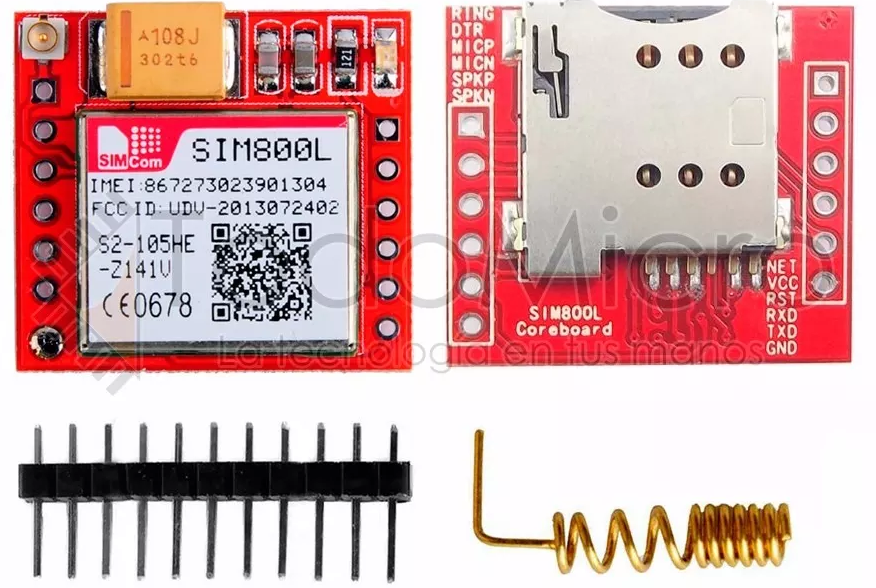
\includegraphics[scale=0.2]{./Figures/sim800.png}
  \caption{Modem SIM800L.}
  \label{fig:sim800l}
\end{figure}

\begin{itemize}
  \item Alimentación: 3.4V a 4.4V (4.0V recomendado)
  \item  CuatriBanda 850/900/1800/1900MHz
  \item  GPRS Multi Slot class 8/10
  \item  Control mediante comandos AT (GSM 07.07 ,07.05 y comandos AT SIMCOM).
\end{itemize}


En la figura \ref{fig:essim800} se puede apreciar el esquemático implementado para la conexión del módem GSM. Éste requiere adaptar los niveles de tensión para interactuar con la CIA-NXP, para el cual utilizamos un max3232.
\begin{figure}[h]
  \centering
  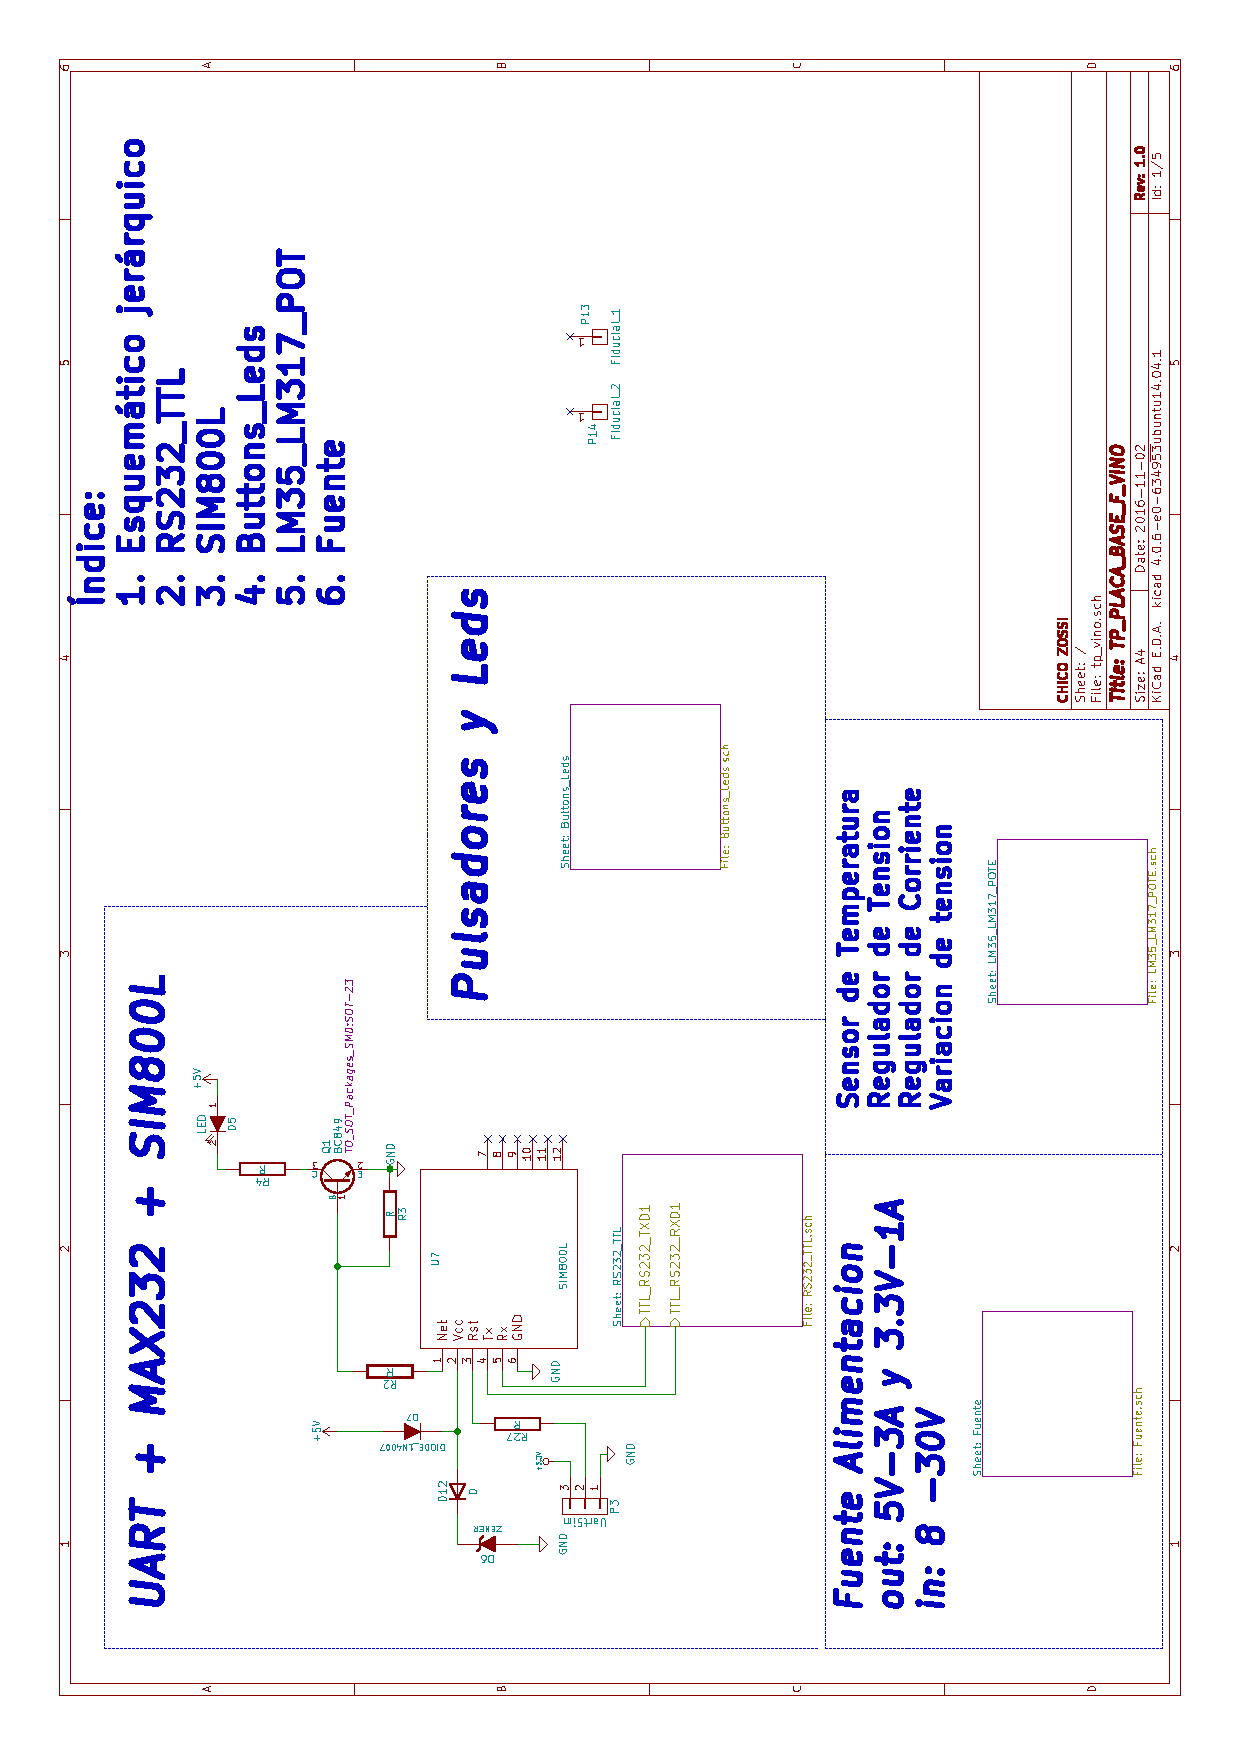
\includegraphics[page=1,scale=0.3,angle=270]{./Figures/schematic.pdf}
  \caption{Módulo sim800l e índice de esquemáticos.}
  \label{fig:essim800}
\end{figure}

Para la alimentación del circuito se utilizó el regulador LM2576. El mismo se tomó de la nota de aplicación el diagrama típico.\footnote{Nota de aplicación Texas Instruments: http://www.ti.com/lit/ds/symlink/lm2576.pdf}
Para regular a 3.3V se utilizó el integrado LM11733 circuito extraído de la nota de aplicación. \footnote{ Texas Instruments: http://www.ti.com/lit/ds/symlink/lm1117.pdf - Capitulo 8 Figura 16 } 
\begin{figure}[h]
  \centering
  \includegraphics[page=3,scale=0.3,angle=270]{./Figures/schematic.pdf}
  \caption{Fuente de alimentación DC/DC.}
  \label{fig:fuente}
\end{figure}

Para lograr la simulación de distintos tipos de sensores, se utilizaron circuitos como se muestra en la figura \ref{fig:temp_tens}  que permiten generar corrientes 4mA a 20mA, variaciones de la tensión, y hasta un sensor de temperatura. Para los circuitos se utilizaron las notas de aplicación de Texas Instruments\footnote{Reguladores de Tensión y Corriente http://www.ti.com/lit/ds/symlink/lm317.pdf - capitulo 8 páginas 12 y 13 y sensor temperatura: http://www.ti.com/lit/ds/symlink/lm35.pdf - 8.2.1 Basic Centigrade Temperature Sensor } 
\begin{figure}[h]
  \centering
  \includegraphics[page=4,scale=0.3,angle=270]{./Figures/schematic.pdf}
  \caption{Regulador de corriente, de tensión y del sensor de temperatura.}
  \label{fig:temp_tens}
\end{figure}

Para concluir, se utilizaron unos circuitos básicos que permiten interactuar en forma simple con el sistema y realizar pruebas de funcionamiento. Los mismos fueron extraídos del esquemático utilizado en el proyecto de la EDU-CIA\footnote{http://www.proyecto-ciaa.com.ar/devwiki/lib/exe/fetch.php?media=desarrollo:edu-ciaa:edu-ciaa-nxp:edu-ciaa-nxp\_color.pdf}

\begin{figure}[h]
  \centering
  \includegraphics[page=5,scale=0.3,angle=270]{./Figures/schematic.pdf}
  \caption{Entradas a leds y salidas de los pulsadores.}
  \label{fig:pul_leds}
\end{figure}

Una vez realizados los esquemáticos, se pasó a la elaboración del PCB. Se realizaron los ruteo necesarios. Y como se puede observar en la siguientes figuras \ref{fig:layer_sup} - \ref{fig:layer_inf} 
\begin{figure}[h]
  \centering
  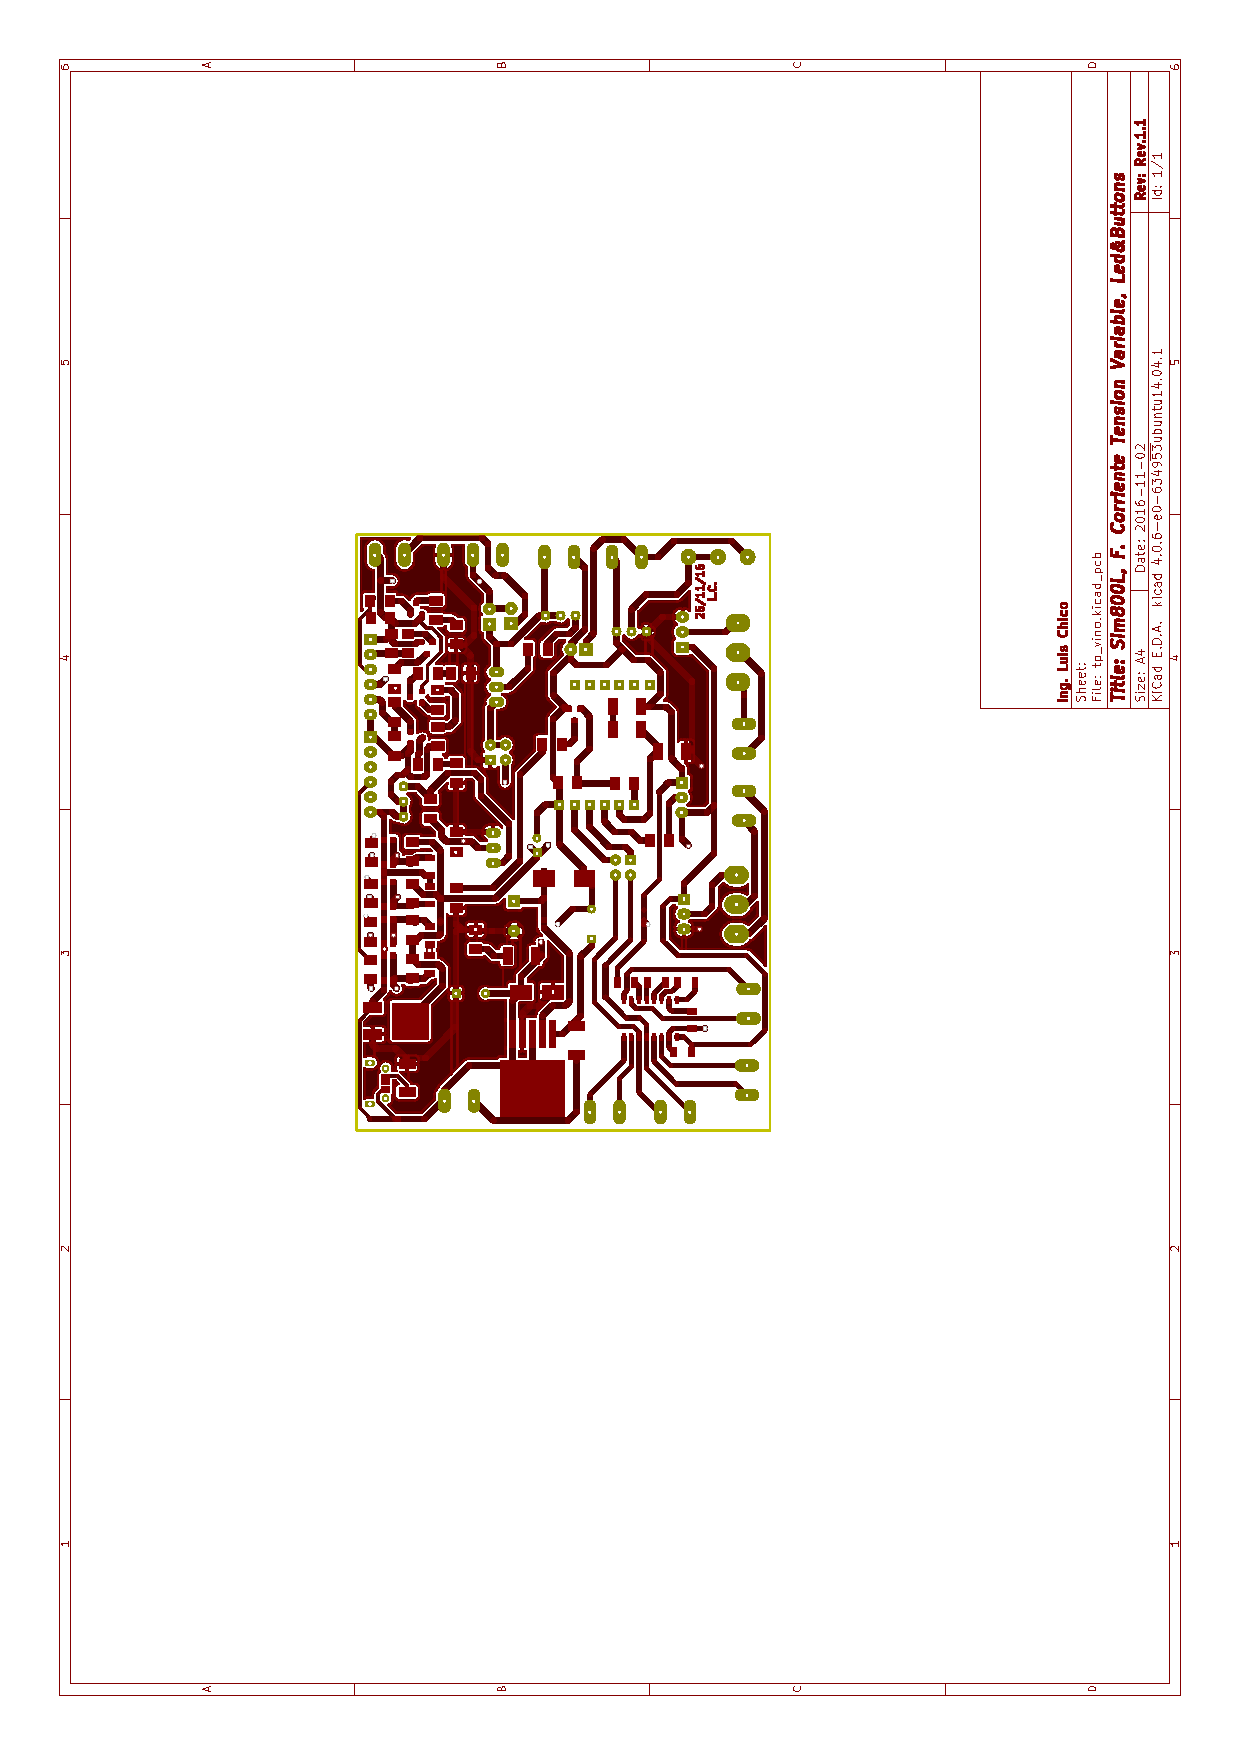
\includegraphics[page=1,angle=270,clip,trim=5.5cm 10cm 7.7cm 8.5cm]{./Figures/pcb_layer.pdf}
  \caption{Capa superior de la placa simulador de sensores.}
  \label{fig:layer_sup}
\end{figure}
\begin{figure}[h]
  \centering
  \includegraphics[page=2,angle=270,clip,trim=5.5cm 10cm 7.7cm 8.5cm]{./Figures/pcb_layer.pdf}
  \caption{Capa inferior de la placa simulador de sensores.}
  \label{fig:layer_inf}
\end{figure}

Realizando una vista previa de como quedaría el esquema y aprovechando el potencial de la herramienta de kicad, se realizó una vista 3D de como quedaría, la que se puede apreciar en la figura \ref{fig:pcb3d}.

\begin{figure}[h]
  \centering
  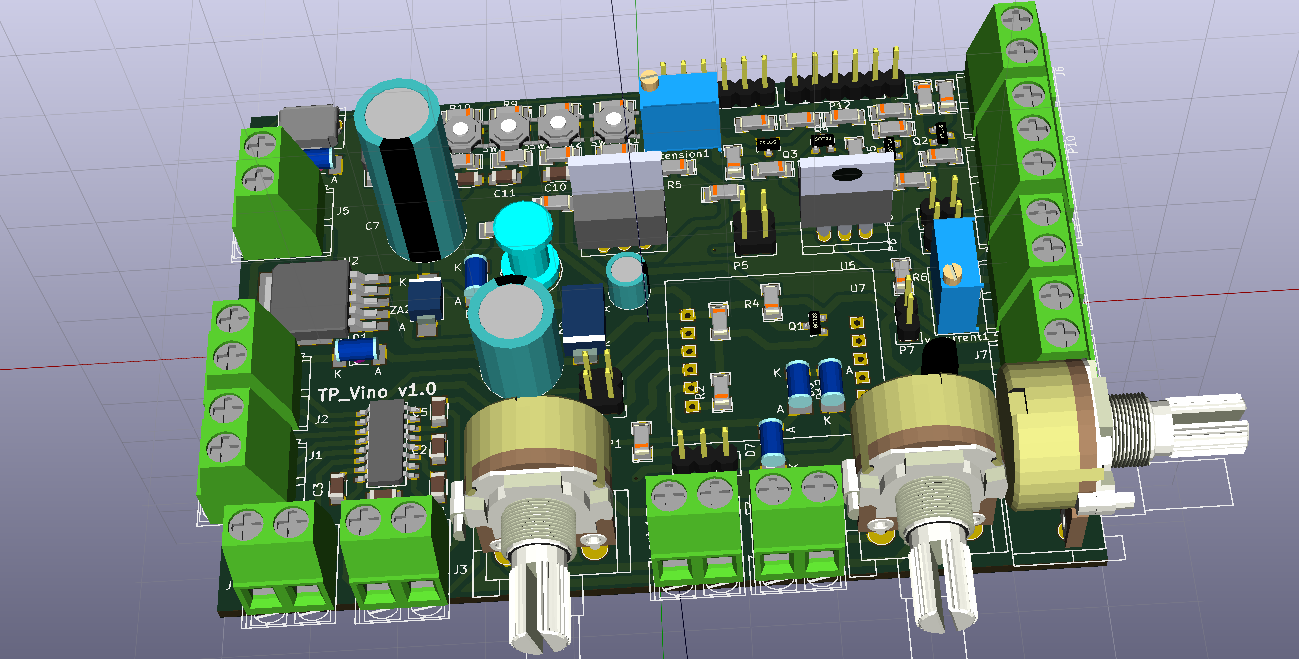
\includegraphics[scale=0.3]{./Figures/pcb_3d.png}
  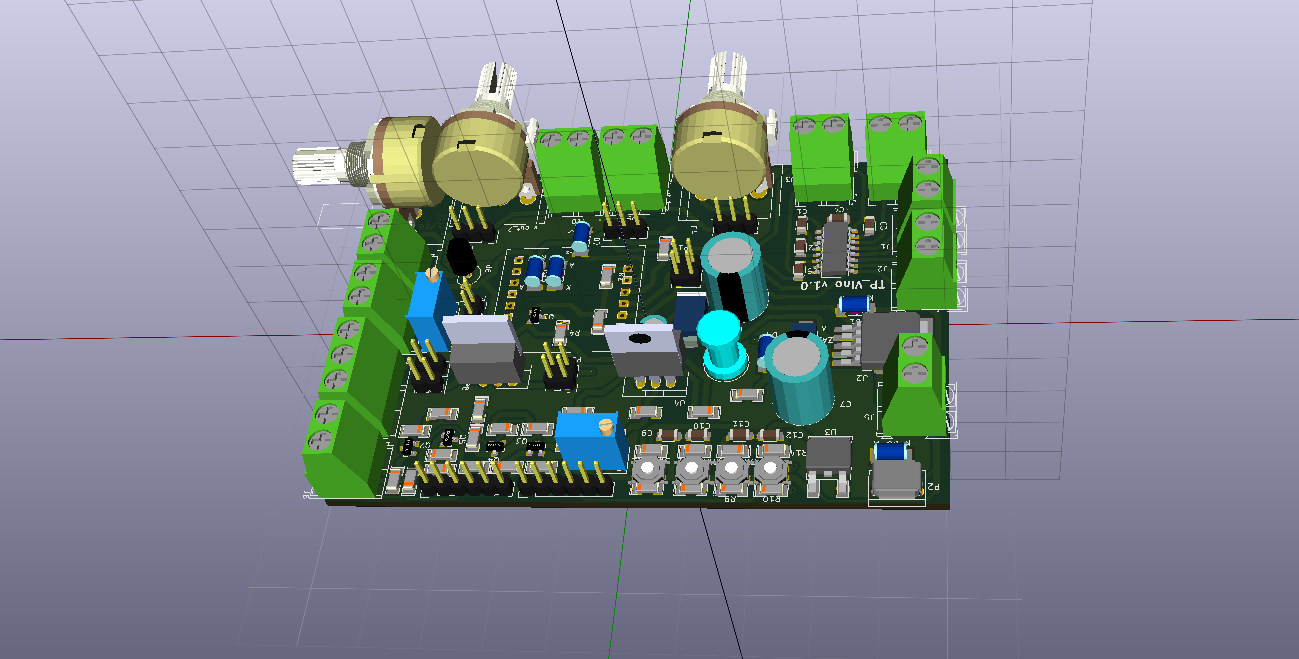
\includegraphics[scale=0.3]{./Figures/pcb_3d_back.png}
  \caption{Placa simulador de sensores 3D.}
  \label{fig:pcb3d}
\end{figure}

No obstante, por cuestiones de tiempo no se llegó a implementar. Simplemente quedó en una primera etapa para una posterior implementación. Se terminó desarrollando una placa experimental que permitió realizar las primeras pruebas. Podemos verla en la siguiente figura \ref{fig:placa_básica}

\begin{figure}[h]
  \centering
  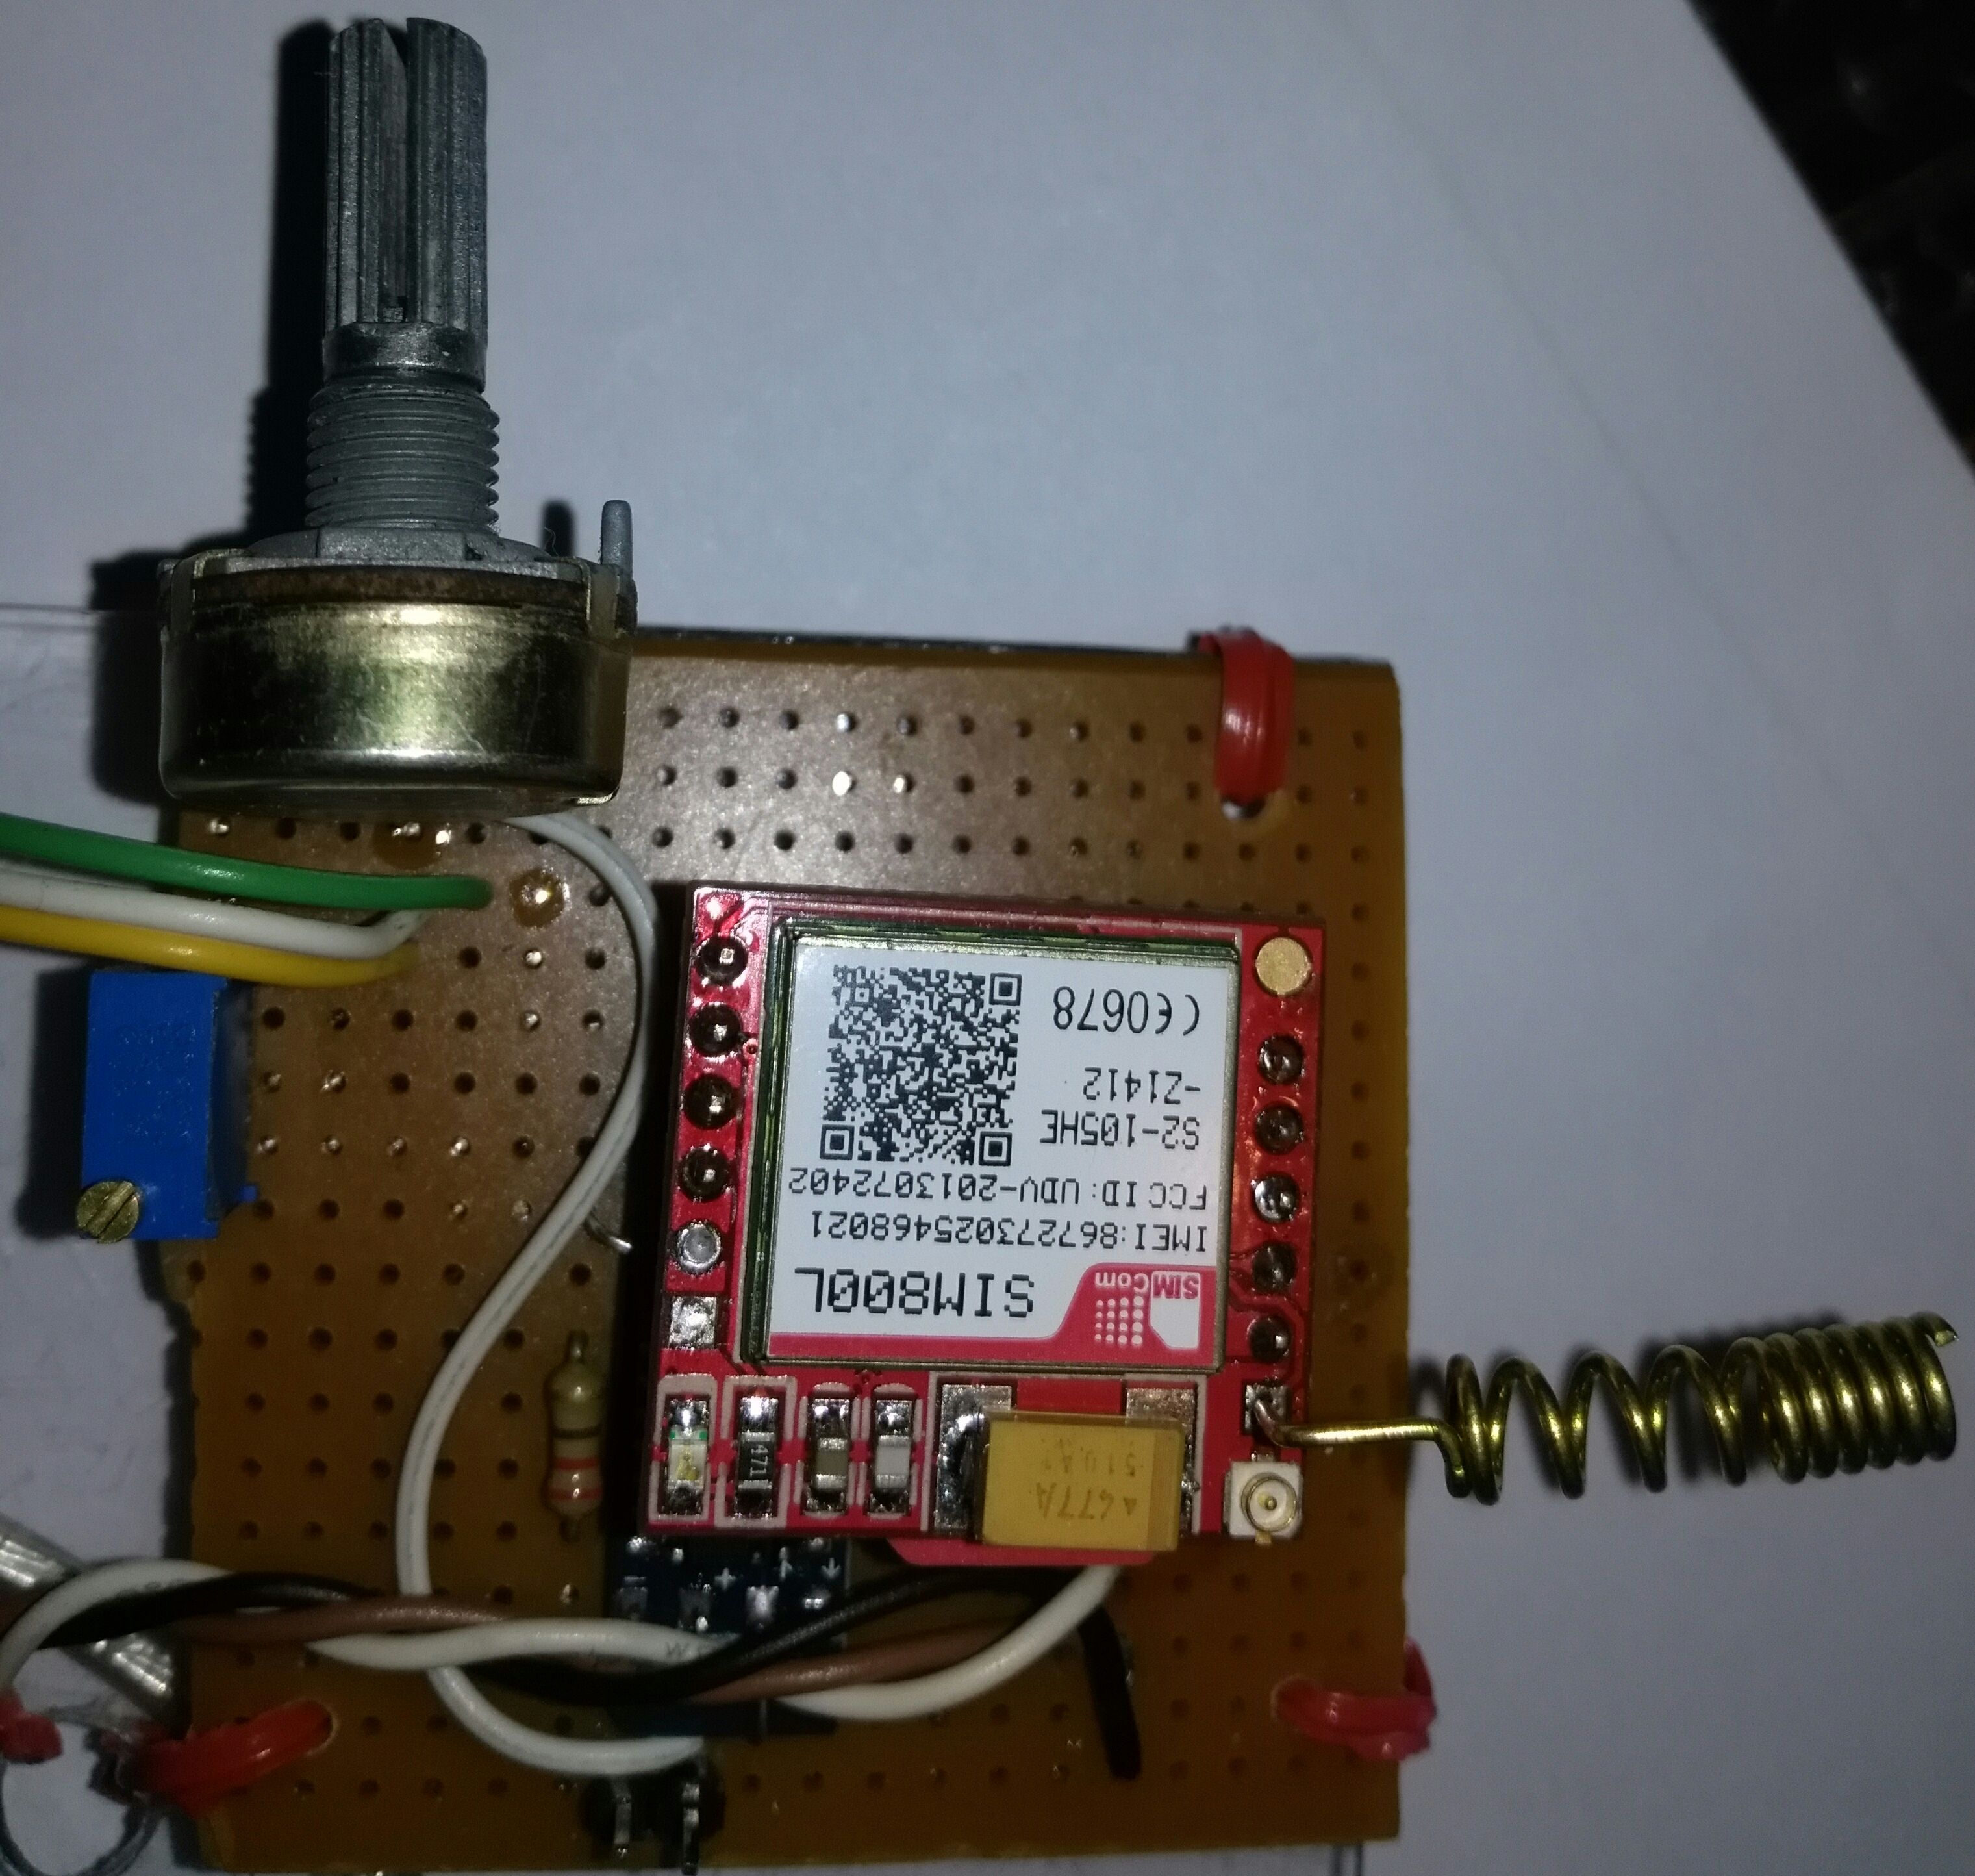
\includegraphics[scale=.03]{./Figures/placa_basica.jpg}
  \caption{Placa de simulación de temperatura y estado de la batería con el modulo SIM800l integrado.}
  \label{fig:placa_básica}
\end{figure}


\section{Software}

Se dividieron las tareas por recursos, una controla el modem, ver Figura \ref{fig:modem_task}.

\begin{figure}[h]
  \centering
  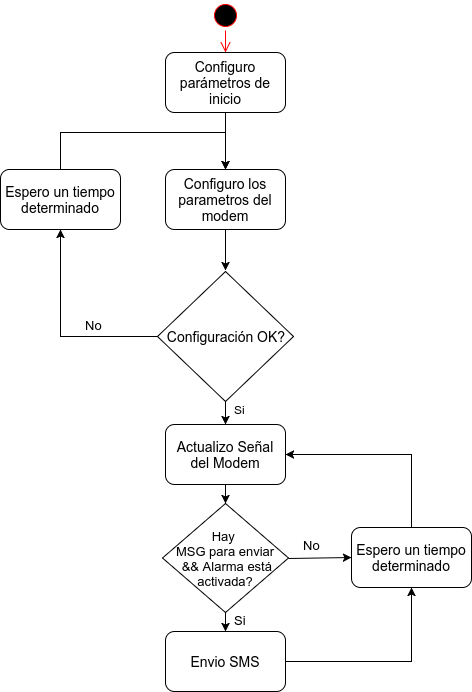
\includegraphics[scale=.4]{./Figures/modem_task.png}
  \caption{Placa de simulación de temperatura y estado de la batería con el modulo SIM800l integrado.}
  \label{fig:modem_task}
\end{figure}



%
%\begin{verbatim}
%\begin{lstlisting}[caption= "un epígrafe descriptivo"]
%
%	las líneas de código irían aquí...
%	
%\end{lstlisting}
%\end{verbatim}
%
%A modo de ejemplo:
%
%\begin{lstlisting}[caption=Pseudocódigo del lazo principal de control.]  % Start your code-block
%
%#define MAX_SENSOR_NUMBER 3
%#define MAX_ALARM_NUMBER  6
%#define MAX_ACTUATOR_NUMBER 6
%
%uint32_t sensorValue[MAX_SENSOR_NUMBER];		
%FunctionalState alarmControl[MAX_ALARM_NUMBER];	//ENABLE or DISABLE
%state_t alarmState[MAX_ALARM_NUMBER];						//ON or OFF
%state_t actuatorState[MAX_ACTUATOR_NUMBER];			//ON or OFF
%
%void vControl() {
%
%	initGlobalVariables();
%	
%	period = 500 ms;
%		
%	while(1) {
%
%		ticks = xTaskGetTickCount();
%		
%		updateSensors();
%		
%		updateAlarms();
%		
%		controlActuators();
%		
%		vTaskDelayUntil(&ticks, period);
%	}
%}
%\end{lstlisting}
%


